\section{Desired model}
\label{sec:desiard_model}

The desired model shall provide a setting for which we can explore fundamental resource and performance properties of the \xcloud{} system paradigm with mobile \ues{}. The mobile \ues{}, radio access network, and service application will subject the \dcs{} to a load characteristic for generic mobile phone traffic and the type of services that plausible might be deployed to the \xcloud{}.

\begin{figure}[tb]
	\centering
	\includegraphics[width=\linewidth]{fig_system_model.eps} 
	\caption{System model}
	\label{fig:system_model}
\end{figure}

As the topology of any future \xcloud{} or proposed forthcoming mobile networks is yet to be determined, in this paper we propose a generic Telecom infrastructure model that disregards generational specific properties such as those found in the physical layer and radio resource load-balancing disciplines. These properties are not system variables at the abstraction level the \xcloud{} needs to be modelled in this paper. Nevertheless, conceivably, and in order to confine the geographic domain of the model, the model adheres to current general LTE cell planing practices \cite{salo2010practical}, see Figure \ref{fig:system_model}.

In order to be able to explore the fundamental effects of mobility on the performance of an \xcloud{} service in the generic case, the model does not adhere to any socio-demographic patterns or urban topologies. In the absence of any geographic bias, the mobile network base stations are uniformly distributed across its 2-dimensional domain.

Similarly, in order to represent the variety of possible services, the service model shall generate traffic that is characteristic for an active, generic, \ue{}. Additionally, the generated traffic shall be provided by a stochastic process that is independent of location.

The mobility model, the service model, and the uniformly distributed mobile network will provide the modelled \dcs{} with a characteristic workload. It is worth reiterating that the traffic load and the characteristics of the service are more relevant to our investigation than specific topological and network properties.

The \dc{} model will host multiple service in VMs that will process the arriving requests corresponding to its service commitment. Additionally, when a VM is migrated between \dcs{} it incurs a load on both \dcs{}. Furthermore, the resources within a \dc{} are shared amongst the hosted VMs. %The amount of compute resources dedicated to one service is thus proportional to the number of services hosted in that \dc{}.  Minute memory management, interference, and cross-talk effects are not fundamental performance properties at this scale and are therefore not modelled.

The above components are reflected in a packets delay composition, see Equation \ref{eq:packet_delay_comp}. Where $LU$ and $LS$ are vectors describing the users associations through its movements based on \rbs and \dc, respectively.

\begin{multline}
D_{M,LU(0)}+D_{N,LU(0) \rightarrow LS(0)} \\ + \sum_{i \in LS[1,N-1]} \left( D_{Mig} + T_{Q,i} + D_{N,i \rightarrow i+1s} \right) + T_{Q,LS(N)} \\ + T_{S,LS(N))} + D_{S,{LS(N)} \rightarrow LU(N)} + D_{M,LU(N)}
\label{eq:packet_delay_comp}
\end{multline}

\begin{multline}
\sum^{N_{init}} T_{init} + \sum^{N_{term}} T_{term} + \sum^{N_{pktser}} T_{ser}  \\ + \sum_{i}^{N_{usrmig}}  \left( \sum_{j}^{N_{pktmig}}  T_{mig} +S\cdot T_{vmmig} \right ) + T_{idle}
\label{eq:vm_util_comp}
\end{multline}
